\subsection*{Tæller}
\label{volumenkontrol-simulering-taeller}

Det er tællerens opgave at holde styr på hvad volumenniveauet er. Der tælles op eller ned når der trykkes på én af de to volumenknapper. Hvor hurtigt der skal tælles bestemmes af det AND'ende signal fra VCO'en og XOR-gaten. VCO'en fungerer som en clock på AND-gaten, mens XOR-signalet sørger for, at det kun er den ene knap der holdes nede. Hvis begge knapper holdes nede, vil XOR-signalet være lavt, og der vil intet signal blive sendt til tælleren. Om der skal tælles op eller ned, styres af et signal fra $\mathrm{volume_{down}}$\fixme{hvad hedder den?} knappen. Hvis denne er nede, som den eneste knap, vil tælleren tælle ned af. Hvis denne ikke er nede, men XOR-signalet stadig er højt, betyder det at den anden knap er nede og tælleren vil derfor tælle op. Tælleren giver et binært output, som danner grundlag for hvad der vises i displayet og hvordan reguleringen af volumen indstilles. Tælleren der benyttes er en 4-bit tæller af typen HEF4516B. Da fire bit ikke er nok skal der bruges to. Yderligere skal der også bruges noget kontrol logik, det er for at sikre tælleren ikke tæller for højt eller lavt og for at styre den anden tæller.

\subsection*{Display}
\label{volumenkontrol-simulering-display}
Indstillingen af volumenkontrollen vises på to 7-segmenter. Dette er valgt, fordi disse er enkle at styre med gate-kredsløb, og det derfor ikke er nødvendigt med en microcontroller, for at styre dem. 

\subsection*{Displaydriver}
\label{volumenkontrol-simulering-display_driver}
Displaydriveren konverterer signalet fra tælleren til et signal der kan vises på de to 7-segment displays. Der konverteres fra tællerens binære output til BCD, Binary-coded decimal, for så at konvertere det til et signal 7-segment displayne kan vise. For delen ved at konvertere til BCD først er at denne konvertering også deler det binære tal op i to, enere og tiere. 

\subsection*{Dæmper}
\label{volumenkontrol-simulering-daemper}
%Volumen kontrollen reguleres ved hjælp af to sæt af 10 modstande, hvor der ved hjælp af 2 skiftere, kan skiftes mellem 100 forskellige konfigurationer. Forholdet imellem de to modstande, der vil sidde serielt, kan udregnes ved hjælp af spændingsdelerformlen, $V_{\mathrm{input}}\cdot\frac{R_2}{R_1+R_2}$. Dette forhold skal ved alle 100 konfigurationer være forskelligt, og ligeligt inddelt, for at volumenkontrollen fungerer. Dettes gøres ved at \fixme{Så mangler vi bare at gøre det}.

Dæmperen er en en analog attenuator, der er sammen sat af to sæt modstands attenuatore adskilt af en buffer. Dæmpningen indstilles ved at ændre hvor signalet tages ud af de to modstands attenuatore, dette styres med en analog multiplekser. Den første attenuatorer består af seks modstande hvor der er en dæmpning på 8 dB mellem hver, den anden attenuatorer består af syv modstande hvor der er en dæmpning på 1 dB mellem hver. Det er således muligt at kombinere de to attenuatorer til at dæmpe signalet mellem 0 og 55 dB, med spring af 1 dB. Diagrammet er afbilledet på figur \ref{fig:volumenkontrol_daemper}. Modstandene er beregnet i appendiks C??.

\begin{figure}[h]
\centering
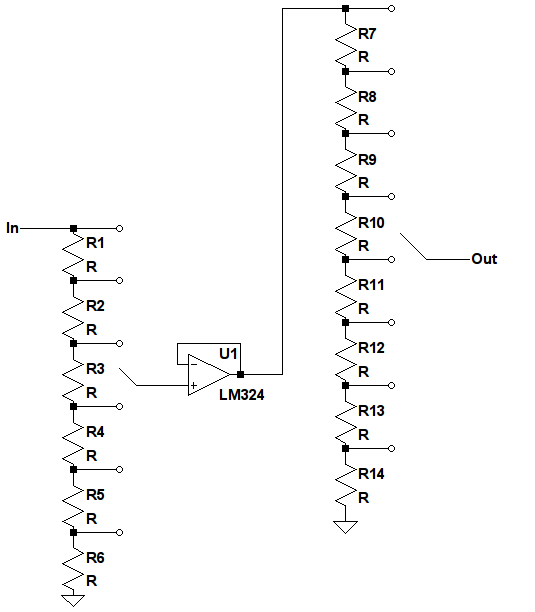
\includegraphics[scale=1]{teknisk/volumenkontrol/daemper.png}
\caption{Diagram over dæmperen}
\label{fig:volumenkontrol_daemper}
\end{figure}

\section{Simulering}
\label{volumenkontrol-simulering}

\section{Accepttest}
\label{volumenkontrol-accepttest}

